\documentclass[11pt,]{article}
\usepackage{lmodern}
\usepackage{amssymb,amsmath}
\usepackage{ifxetex,ifluatex}
\usepackage{fixltx2e} % provides \textsubscript
\ifnum 0\ifxetex 1\fi\ifluatex 1\fi=0 % if pdftex
  \usepackage[T1]{fontenc}
  \usepackage[utf8]{inputenc}
\else % if luatex or xelatex
  \ifxetex
    \usepackage{mathspec}
  \else
    \usepackage{fontspec}
  \fi
  \defaultfontfeatures{Ligatures=TeX,Scale=MatchLowercase}
\fi
% use upquote if available, for straight quotes in verbatim environments
\IfFileExists{upquote.sty}{\usepackage{upquote}}{}
% use microtype if available
\IfFileExists{microtype.sty}{%
\usepackage{microtype}
\UseMicrotypeSet[protrusion]{basicmath} % disable protrusion for tt fonts
}{}
\usepackage[left=2cm, right=2cm, top=2cm, bottom=2cm]{geometry}
\usepackage{hyperref}
\PassOptionsToPackage{usenames,dvipsnames}{color} % color is loaded by hyperref
\hypersetup{unicode=true,
            pdftitle={How Americans' Time Use Patterns Have Changed From 2003 to 2017},
            colorlinks=true,
            linkcolor=Maroon,
            citecolor=Blue,
            urlcolor=blue,
            breaklinks=true}
\urlstyle{same}  % don't use monospace font for urls
\usepackage{graphicx,grffile}
\makeatletter
\def\maxwidth{\ifdim\Gin@nat@width>\linewidth\linewidth\else\Gin@nat@width\fi}
\def\maxheight{\ifdim\Gin@nat@height>\textheight\textheight\else\Gin@nat@height\fi}
\makeatother
% Scale images if necessary, so that they will not overflow the page
% margins by default, and it is still possible to overwrite the defaults
% using explicit options in \includegraphics[width, height, ...]{}
\setkeys{Gin}{width=\maxwidth,height=\maxheight,keepaspectratio}
\setlength{\emergencystretch}{3em}  % prevent overfull lines
\providecommand{\tightlist}{%
  \setlength{\itemsep}{0pt}\setlength{\parskip}{0pt}}
\setcounter{secnumdepth}{0}
% Redefines (sub)paragraphs to behave more like sections
\ifx\paragraph\undefined\else
\let\oldparagraph\paragraph
\renewcommand{\paragraph}[1]{\oldparagraph{#1}\mbox{}}
\fi
\ifx\subparagraph\undefined\else
\let\oldsubparagraph\subparagraph
\renewcommand{\subparagraph}[1]{\oldsubparagraph{#1}\mbox{}}
\fi

%%% Use protect on footnotes to avoid problems with footnotes in titles
\let\rmarkdownfootnote\footnote%
\def\footnote{\protect\rmarkdownfootnote}

%%% Change title format to be more compact
\usepackage{titling}

% Create subtitle command for use in maketitle
\newcommand{\subtitle}[1]{
  \posttitle{
    \begin{center}\large#1\end{center}
    }
}

\setlength{\droptitle}{-2em}

  \title{\textbf{How Americans' Time Use Patterns Have Changed From 2003 to 2017}}
    \pretitle{\vspace{\droptitle}\centering\huge}
  \posttitle{\par}
  \subtitle{Group July}
  \author{}
    \preauthor{}\postauthor{}
      \predate{\centering\large\emph}
  \postdate{\par}
    \date{26 November 2018}

\usepackage{booktabs}
\usepackage{longtable}
\usepackage{array}
\usepackage{multirow}
\usepackage[table]{xcolor}
\usepackage{wrapfig}
\usepackage{float}
\usepackage{colortbl}
\usepackage{pdflscape}
\usepackage{tabu}
\usepackage{threeparttable}
\usepackage{threeparttablex}
\usepackage[normalem]{ulem}
\usepackage{makecell}

\usepackage{animate}
\usepackage{indentfirst}

\begin{document}
\maketitle

\hypertarget{introduction}{%
\section{Introduction}\label{introduction}}

The aim of this report is to discover how Americans' time use patterns
have changed over the last 15 years, through discovering and analysing
long-term trends over the years of 2003 to 2017. The datasets
{[}\protect\hyperlink{ref-atusdatasets}{1}{]} used to tackle this
comprise some of the results of the American Time Use Survey (ATUS)
{[}\protect\hyperlink{ref-ATUS}{2}{]}. ATUS respondents were interviewed
once about how they spent their time on the previous day, where they
were, and whom they were with. The survey records the time spent on 431
different activities that are grouped into 17 different categories. In
the analysis these categories will often be referred to by a variable
beginning with \texttt{tu} followed by a two-digit \emph{category
number}. The meaning of each category number and identifications for the
rest of the variables can be found in the lexicon and data dictionary
files which are available on the
\href{https://www.bls.gov/tus/lexiconnoex0317.pdf}{ATUS website}.

The \href{https://www.bls.gov/tus/charts.htm}{Bureau of Labor Statistics
website} provides a number of charts looking at the 2017 annual averages
for these categories. This report provides a more definitive conclusion
on how time use patterns changed over the period, evidenced with
statistical investigation of the data. The findings offer in-depth
explanations as to where some of the biggest fluctuations are and
suggests possible reasons for these fluctuations. Limitations to the
analysis are noted where appropriate and these must be taken into
account when performing any further analysis or summaries, and mentioned
alongside any conclusions.

Usually when analysing data, statisticians will split the dataset into
training data and validation data. This ensures that any conclusions
drawn from exploratory data analysis (EDA) on the training data can be
verified using the remaining ``unseen'' validation data. The analysis
performed for this report follows this technique, splitting the data
approximately in half to provide continuity and robustness in model
training. The split was done by selecting even and odd months for
training and validation data respectively, in order to ensure that
seasonality did not cause incorrect rejections of hypotheses posed based
upon the EDA, as well as ensuring there were no uneven gaps in the data
which may lead to a loss of clarity in plotting. This split also allowed
for conformity to one of the project requirements that the month of July
was to be excluded initially and used for validation.

\hypertarget{the-compelling-change-in-caring-for-helping-non-hh-members}{%
\section{The Compelling Change in Caring for \& Helping Non-HH
Members}\label{the-compelling-change-in-caring-for-helping-non-hh-members}}

\hypertarget{exploratory-data-analysis}{%
\subsection{Exploratory Data Analysis}\label{exploratory-data-analysis}}

In order to effectively discover trends in the data whilst still being
able to validate these trends, the data was split as mentioned before by
taking alternate months and assigning them to training and validation
data sets respectively. The even months were used throughout the EDA in
this part of the report as well as the EDA in the
\protect\hyperlink{howthetimespentontraditionallygenderedactivitieshasconvergedasgenderroleshavebrokendown}{later
part}.

The ATUS dataset records time spent on activities in minutes. When all
17 variables are plotted it appears that there is more variation in the
proportion of American's partaking in activities than there is in the
raw time use values. Therefore, the EDA in this section initially
focussed on looking at how the proportion of American's partaking in the
17 categories of activities has changed. The following table gives a
summary of some of these changes. The activities included are those with
a percentage change of over 10\% and a variance greater than 0.5, i.e
those which are deemed to be of interest for further analysis and
exploration.

\begin{table}[!h]

\caption{\label{tab:Weighted Means Variance and Percentage Change Table}Change in Participation of Activities}
\centering
\begin{tabu} to \linewidth {>{\raggedright}X>{\raggedleft}X>{\raggedleft}X>{\raggedleft}X>{\raggedleft}X>{\raggedleft}X}
\toprule
Measure & tu04 & tu08 & tu13 & tu14 & tu16\\
\midrule
Variance & 2.54 & 0.89 & 1.44 & 0.60 & 1.93\\
\% Change & -32.11 & -26.46 & 10.17 & 12.32 & -24.08\\
\bottomrule
\end{tabu}
\end{table}

It is immediately clear that the most compelling change out of the 17
activity groups, over the period, is in \emph{Caring for \& Helping
Non-household (Non-HH) Members} represented by \texttt{tu04} in the
data. However, without some further exploration, this is arguably
uninteresting.

When fitting a linear model, the method of best subsets with \emph{Year}
forced in as a variable tells us that the most significant variables to
predict the proportion of American's spending time \emph{Caring for \&
Helping Nonhousehold (NonHH) Members} are \emph{Sex} and \emph{Number of
Household Children}. Ths model is not sufficient to accurately predict
\texttt{tu04} participation, however it does give a good idea as to what
is causing the change over the period 2003 to 2017.

The non-negative, non-linear nature of the continuous activity data also
means a more complex model would be suitable. An \(F\)-test shows such a
complex model which incorporates \emph{Sex} is a significant improvement
over such a model which doesn't include it. This confirms the belief
that is has a significant effect on participation in caring for \&
helping non-household members.

The plot below is a graphical interpretation of the model, built on the
training data, with the average number of household children, for each
group of the population, displayed as \textbf{bars}. Participation
percentage in caring for \& helping non-household members is displayed
as smooth lines.

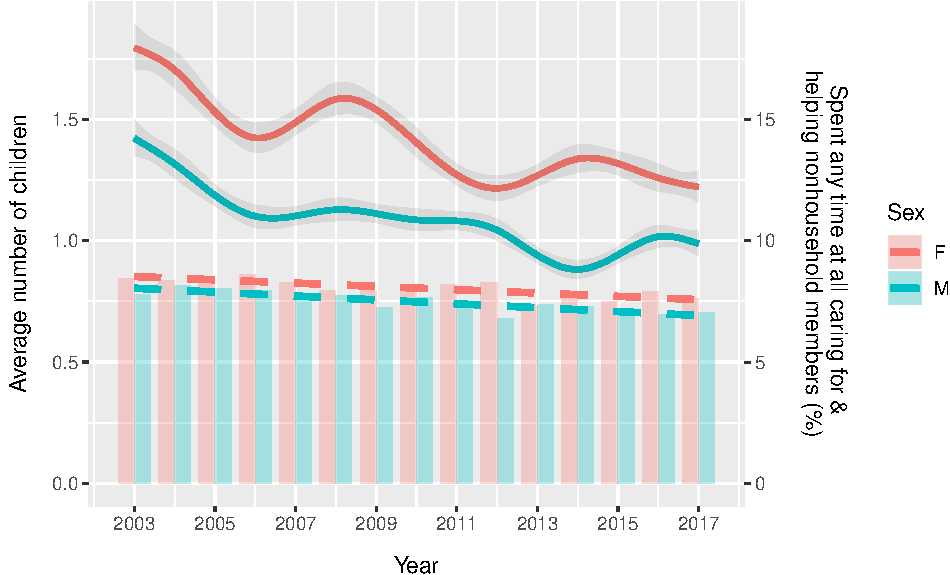
\includegraphics{Final_Final_Report_files/figure-latex/part_tu04 Sex Plot with Number of Children-1.pdf}

The key observation is that, as the table suggested, over the period the
participation in caring for \& helping non-household members has
decreased for both men and women. Building a linear model using
\emph{Sex} and \emph{Year} and performing a \(t\)-test confirms this.
There also appears to be a link between participation in caring for \&
helping non-household members and the number of household children.
Updating the spline curve model to include the number of household
children and then again testing this hypothesis with a t-test confirms
this is also the case. Looking at the graph, fluctuations in the average
number of household children, on the whole seem to be followed by but if
we check the correlations between them, they show this link is fairly
weak (0.65 for Men and 0.49 for Women), suggesting there must be further
reasons for this change; possibly not measured in this dataset.
Therefore, further analysis must be done before a statistically sound
conclusion on the causation of the changes can be made.

\hypertarget{validation}{%
\subsection{Validation}\label{validation}}

As in the EDA, but this time formally, a linear model is built using
\emph{Sex} and \emph{Year} and a \(t\)-test performed. It gives a
\(p\)-value \(< 0.05\) (quite a bit less in fact). This means there is
sufficient evidence to conclude that the proportion of American's who
participate in caring for \& helping non-household members has in fact
decreased over the period 2003-2017 as suggested by the EDA.

The initial thoughts about the link with number of household children,
from the EDA, again needed to be tested. A new model of the same
structure was built. Another formal t-test could then be completed on an
update of this model which includes the number of household children.

With a \(p\)-value \(< 0.05\), this test confirms this belief in the
validation data.

We have now verified that the conclusions suggested by the EDA are
correct: the percentage of American's who partake in caring for \&
helping non-household members has decreased over the period from 2003 to
2017. There also seems to be a link between the number of children in
the household and the participation percentage. The plot below gives a
graphical interpretation of changes using a model fit on all the data,
only excluding those responses taken in July for each year.

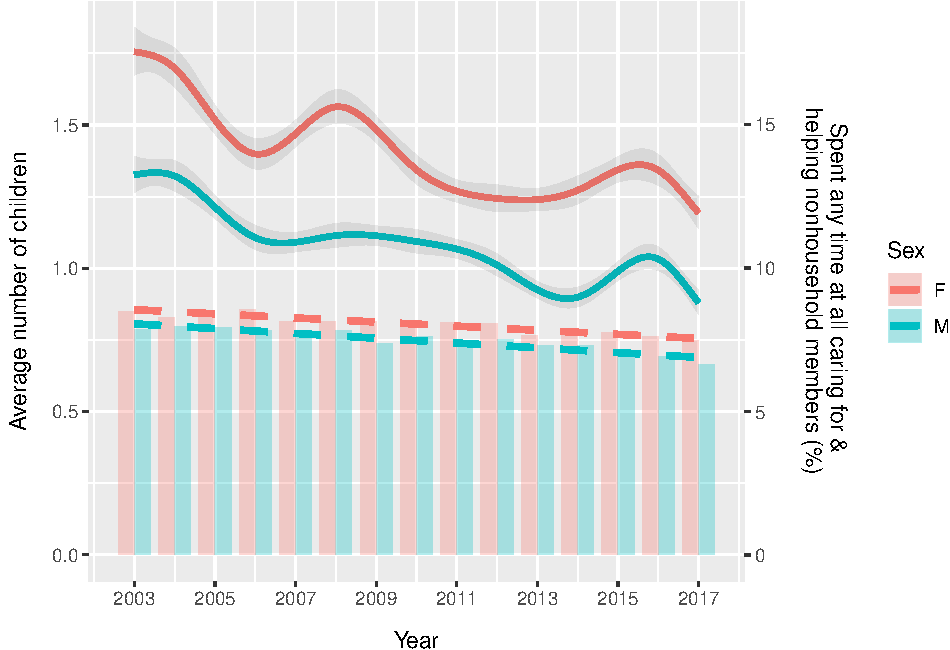
\includegraphics{Final_Final_Report_files/figure-latex/part_tu04 Sex Plot with Number of Children Plotting-1.pdf}

\hypertarget{how-the-time-spent-on-traditionally-gendered-activities-has-converged-as-gender-roles-have-broken-down}{%
\section{How The Time Spent on Traditionally Gendered Activities has
Converged as Gender Roles have Broken
Down}\label{how-the-time-spent-on-traditionally-gendered-activities-has-converged-as-gender-roles-have-broken-down}}

The discussion surrounding social division between genders in terms of
roles and responsibilities has consistently been a major news topic in
recent years. This debate has been fuelled by a new wave of feminism, as
well as a number of different social media campaigns such as
\emph{`\#MeToo'} and \emph{`Times Up'}. Both of these movements aimed to
address commonplace sexual harassment and discrimination, empowering
women to take back control. Given this current social climate, it was
decided that an interesting area of the ATUS data to focus on would be
long-term changes in time use for different sexes. Specifically, areas
of time use where pre-existing gender roles are present were examined.

\hypertarget{exploratory-data-analysis-1}{%
\subsection{Exploratory Data
Analysis}\label{exploratory-data-analysis-1}}

Talcott Parsons' {[}\protect\hyperlink{ref-10.2307ux2f2085686}{3}{]}
study on gender roles - published in the 1950's - compared traditional
gender roles with more liberal alternatives. A simplified version of
this strictly traditional view of gender roles is detailed in the table
below.

\begin{table}[H]

\caption{\label{tab:unnamed-chunk-2}Traditionally Perceived Gender Activities}
\centering
\begin{tabular}[t]{lr}
\toprule
Male Activites & Female Activities\\
\midrule
Working & Housework\\
House Maintenance & Food Preparation\\
Vehicle Maintenance & Childcare\\
\bottomrule
\end{tabular}
\end{table}

The liberal viewpoint discussed by Parsons suggests an equal balance of
time for the genders in these roles. Whilst this study was developed
over 50 years ago, a preliminary look at the data confirmed that, in
2003, a complete transition to the liberal viewpoint had not occurred.
Therefore, it was decided to investigate whether the time use of these
specific activities was converging to equality or remaining stationary
with noticeable differences between genders. In order to do this as
rigorously and objectively as possible, weighted averages were
calculated amongst each demographic to best represent how different
groups of peoples' time uses had changed over time and to make up for
any inconsistencies in the data.

Following some initial exploration of the data and breaking down the
respondents into different generations
{[}\protect\hyperlink{ref-generations}{4}{]}, another layer of
complexity to the analysis was developed. Splitting the data by age
allowed for further hypotheses regarding progression through convergence
of time use for both genders in the areas discussed above; it would
perhaps be assumed that younger people would be more progressive in this
respect. Using this generational approach provided a way of tracking a
population over time without having to arbitrarily pick age categories.
A small number of participants fell outside of these ranges, however,
these represented only a small number of participants and so were added
to the next nearest generation (e.g.~if a participant was born in 1998,
they would be added to the \emph{Millennials} generation).

\begin{table}

\caption{\label{tab:unnamed-chunk-3}Generations}
\centering
\begin{tabular}[t]{lr}
\toprule
Generation & Birth Years\\
\midrule
Silent Generation & 1928 - 1945\\
Baby Boomers & 1946 - 1964\\
Generation X & 1965 - 1980\\
Millennials & 1981 - 1996\\
\bottomrule
\end{tabular}
\end{table}

For each of the activities, a suitable generalized linear model was
developed using \emph{Sex}, \emph{Year} and \emph{Generation} as
parameters. The values used to predict each model were constructed using
the weighted mean formula provided in the \textbf{ATUS User's Guide},
available online in the ATUS Survey Documentation. Splines were added to
the model for each year and graphical representations were produced.
These graphical representations allowed for hypotheses to be formulated
regarding the change in time use for these gender-stereotyped variables
over the period. It was from these hypotheses that validation could then
be carried out to see if the conclusions were consistent and thus
whether the trend was likely to have substance behind it.

It was decided to plot a line for each of the genders despite the
interest of the analysis being focussed on the difference \emph{between}
the genders. This is because having lines to associate with each gender
is likely more clear to the reader and can more intuitively show any
narrowing of the gap between genders for the variables of interest.

As far as the hypotheses there are to validate, they can be summarised
similarly for each variable: as first posed in the aforementioned 1950's
study, it is likely that social changes will lead to an erosion of
gender roles. The EDA suggested that this erosion has continued from
2003 to 2017 and so validation is required to attempt to confirm that
the difference in time use for the relevant variables has indeed
decreased as time has continued.

\hypertarget{validation-1}{%
\subsection{Validation}\label{validation-1}}

In order to validate the trends found in the EDA, the same approach to
that taken in the first part of the report was followed: splitting the
data set initially and using the unseen half to validate the
observations and hypotheses made above. The validation data was then put
through the same models used in the EDA and the hypotheses validated
observationally. In addition to this more intuitive technique of
validation, statistical \(t\)-testing was carried out to ensure
significance in the shrinking difference between the two genders for the
variables of interest. The models below showcase the results of the
analysis after validation was carried out, plotting all of the data with
the exception of July as required in the specification of this report.
Despite using 11 months of the data here, it is critical to reiterate
that all of the EDA and validation was carried out on entirely separate
6 month subsets of each year to ensure validity of the conclusions and
testing.

\hypertarget{working}{%
\subsubsection{Working}\label{working}}

The plots below show the change in working patterns between three
different generations. The \emph{Silent Generation} have been excluded
from this plot as - by 2010 - the youngest of this generation will be
65. At this age, most will have retired and as such the plot is not
likely to be very informative. Furthermore, the same scale is used for
each graph (for ease of comparison), so including the \emph{Silent
Generation} would adversely affect the quality of comparison between the
more informative generations.

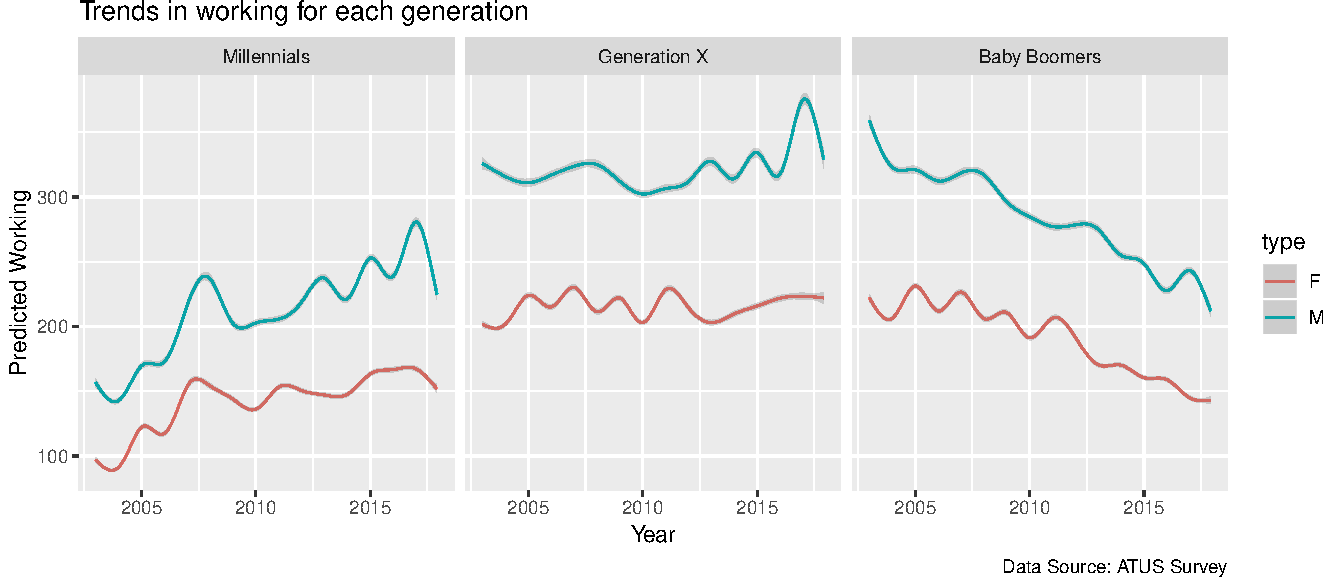
\includegraphics{Final_Final_Report_files/figure-latex/unnamed-chunk-4-1}
It can be seen that year on year there has been a slight contraction,
especially visible in \emph{Generation X} when the peak around 2016 is
ignored. It is clear that generationally, working hours follow a fairly
standard trajectory, peaking for people in their middle ages.
\emph{Millennials} have seen a steady increase in their time spent
working as would be expected for people in that age range; the genders
seem to have a much smaller gap between them when compared with
\emph{Generation X} though, which is testament to part of the hypothesis
made above regarding progressive social norms propagating through
younger generations.

\hypertarget{house-maintenance-and-vehicle-maintenance}{%
\subsubsection{House Maintenance and Vehicle
Maintenance}\label{house-maintenance-and-vehicle-maintenance}}

For both of these variables, it was decided that the participation rate
was too low to warrant deeper analysis. Whilst the EDA findings
suggested that there existed a separation in gender, with men spending
more time on both of these activities, the participation rates of around
3\% for both reflected that these were more uncommon activities. As
such, it was decided that there was not enough data to reflect the time
spent in a suitable linear model; variance was much greater amongst the
lower valued variables and these particular fluctuations did not seem to
follow a clear long term trend.

\hypertarget{housework}{%
\subsubsection{Housework}\label{housework}}

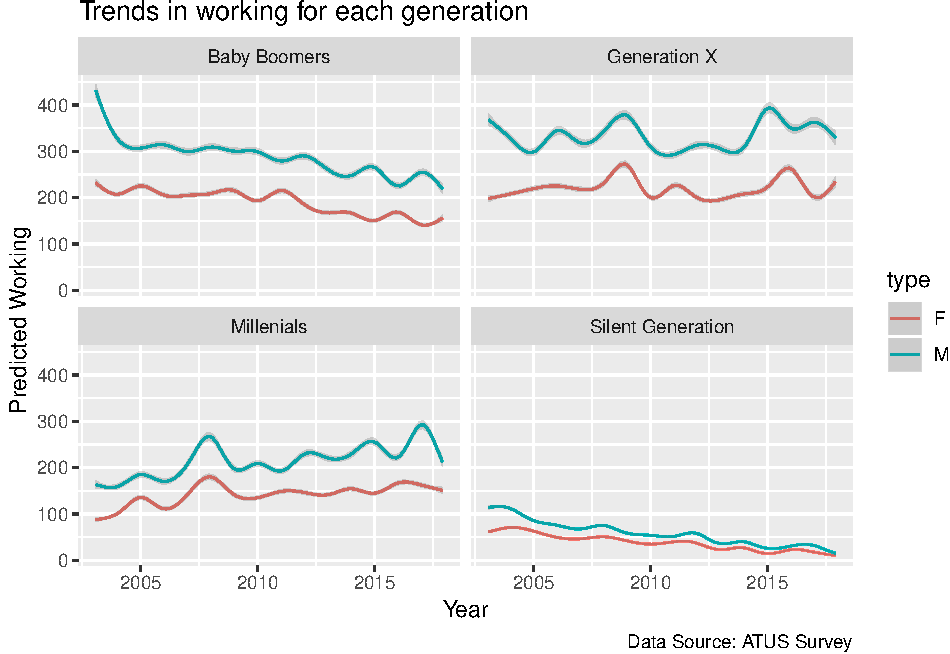
\includegraphics{Final_Final_Report_files/figure-latex/unnamed-chunk-5-1}

The graphs above show that for all generations, except for
\emph{Millennials}, there has been a decrease in the gap in time spent
on housework between men and women. This is as a result of men spending
more time and women spending less time on housework, although the
decrease for women is sharper than the increase for men. This trend is
reflected clearly in \emph{Generation X}, the second youngest
generation. However, there is also strong evidence for this trend in the
\emph{Silent Generation} despite the slight divergence in 2016. On the
other hand, the gap seems to have increased slightly for
\emph{Millennials} - both sexes are increasing the amount of time spent
on housework, but the increase is not as great for men. Notably,
\emph{Millennials} also spend substantially less time doing housework
than the other generations, with the highest point being around 45
minutes per day (women in 2016), compared to around 62 in \emph{Baby
Boomers} and \emph{Generation X} and 72 minutes in the \emph{Silent
Generation}. Therefore, whilst the gap is increasing for
\emph{Millennials}, it is still smaller than all of the other
generations at around 25 minutes. Comparatively, the \emph{Silent
Generation's} gap started at over 50 minutes in 2003 and has decreased
to just under 45.

\hypertarget{food-preparation}{%
\subsubsection{Food Preparation}\label{food-preparation}}

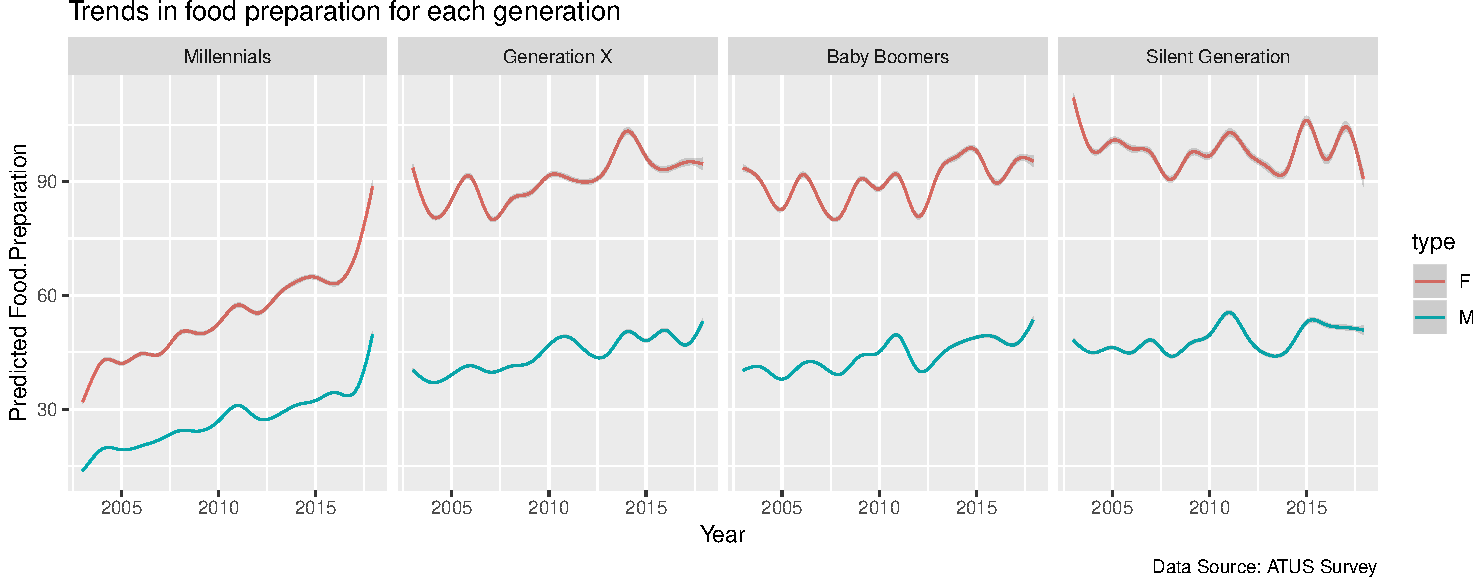
\includegraphics{Final_Final_Report_files/figure-latex/unnamed-chunk-6-1}

The graphs above show a very similar trend to \texttt{Housework} in the
sense that the gap is decreasing and that all generations apart from
\emph{Millennials} spend a similar amount of time in general on this
activity. However, the difference with this activity is that for
\emph{Baby Boomers} and \emph{Generation X}, women are actually spending
more time on this activity than they were previously - the decrease in
the gap is as a result of a sharper increase for men perhaps as cooking
and spending time at home is more normalised in society. For
\emph{Millennials}, the situation is slightly different: both sexes are
spending more time on this activity but the increase for both is at an
equal rate and so the gap is maintained. The \emph{Silent Generation} is
the generation showing the biggest decrease in the gap between sexes;
this is due to the decrease for women and an increase for men, although
this generation started off with the highest values for both sexes. This
generation is likely to have more free time to begin with an thus
exhibit more initial variance but then reflect the changes in society
more clearly as cooking as an activity becomes more common amongst men.

\hypertarget{childcare}{%
\subsubsection{Childcare}\label{childcare}}

For similar reasons to working, the \emph{Silent Generation} has been
excluded from this section as most of the people in this age range are
unlikely to have any household children of their own.

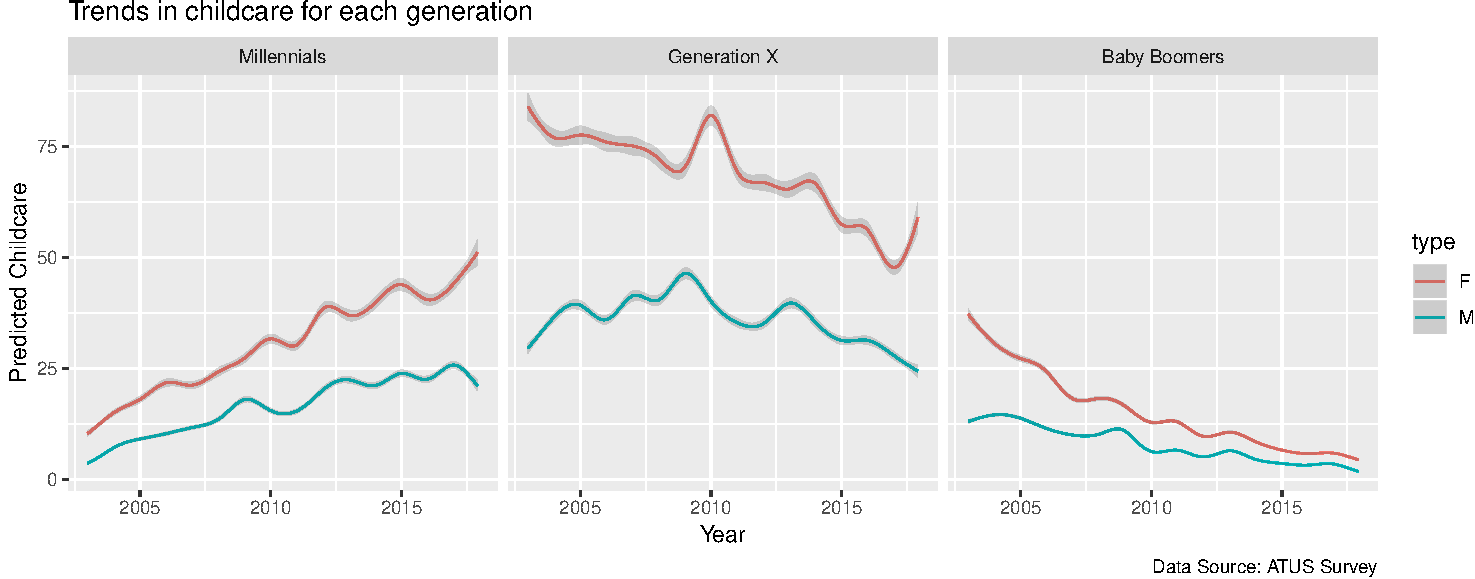
\includegraphics{Final_Final_Report_files/figure-latex/unnamed-chunk-7-1}

These graphs show perhaps the greatest change in gender roles. The data
for \emph{Baby Boomers} and the \emph{Silent Generation} shows very
little, most likely as the variables included in childcare relate only
to caring for household children, where a child is defined as someone
below the age of 18. It is unlikely that many people within these
generations would have children living with them at this age (in fact
checking the data confirms that, in 2017, only 9\% met this criteria).
Furthermore, at this age their children are likely to be older and
require less constant care as they become more independent. Therefore,
the other generations - \emph{Millennials} and \emph{Generation X} -
exhibit more interesting trends. For reasons similar to the older
generations, the drop off in childcare at the end of \emph{Generation X}
can likely be explained as children mature. However, it is important to
note that the drop off for women is sharper than it is for men, leading
to a convergence in the weighted means for both. The gap has decreased
substantially, from 50 minutes per day in 2003 to less than half that,
around 20 minutes in 2017. This could further be attributed to the
decrease in working time for this generation, noted above. The
\emph{Millennials} on the other hand exhibit an increase year on year
for activities in childcare. Whilst the gap increases slightly over
time, it doesn't ever reach a similar point to that of \emph{Generation
X}, with the biggest difference being around 40\% compared to 60\%.

\hypertarget{conclusions}{%
\section{Conclusions}\label{conclusions}}

Will do tomorrow morning, someone else feel free to have a go.

\hypertarget{limitations-of-the-data}{%
\subsection{Limitations of the Data}\label{limitations-of-the-data}}

One of the major limitations imposed on this research is the length of
the period within which the data was gathered: 15 years is a short
amount of time to observe trends amongst such a large population. This
meant that often the data had to first be subsetted or transformed as no
immediate trends were visible at the surface, this led to sporadic
subset size (as mentioned with respect to \emph{Vehicle} and \emph{House
Maintenance}) due to the number of filters required to get down to the
demographics that were desirable to investigate.

\parindent0pt

\hypertarget{references}{%
\section*{References}\label{references}}
\addcontentsline{toc}{section}{References}

\hypertarget{refs}{}
\leavevmode\hypertarget{ref-atusdatasets}{}%
{[}1{]} ``ATUS datasets.''
\url{https://www.bls.gov/tus/datafiles_0317.htm}.

\leavevmode\hypertarget{ref-ATUS}{}%
{[}2{]} Bureau of Labor Statistics, ``The american time use survey.''
\url{https://www.bls.gov/tus/}, 2017.

\leavevmode\hypertarget{ref-10.2307ux2f2085686}{}%
{[}3{]} T. Parsons, ``Age and sex in the social structure of the united
states,'' \emph{American Sociological Review}, vol. 7, no. 5, pp.
604--616, 1942 {[}Online{]}. Available:
\url{http://www.jstor.org/stable/2085686}

\leavevmode\hypertarget{ref-generations}{}%
{[}4{]} ``Millennials projected to overtake baby boomers as america's
largest generation.''
\url{http://www.pewresearch.org/fact-tank/2018/03/01/millennials-overtake-baby-boomers/}.


\end{document}
